\documentclass[titlepage]{article}
\usepackage[utf8]{inputenc}
\usepackage{color}   %May be necessary if you want to color links
\usepackage{hyperref}
\usepackage[french]{babel}
\usepackage{cite}
\usepackage{graphicx}

\usepackage[square,numbers]{natbib}
\bibliographystyle{abbrvnat}

\hypersetup{
	colorlinks=true, %set true if you want colored links
	linktoc=all,     %set to all if you want both subsections and subsubsections linked
	linkcolor=blue,  %choose some color if you want links to stand out
}
\title{Arbre comportementaux pour le contr\^ole de mission}
\author{
	Derrien Martial \\
	\and
	Madec Antoine \\
	\and
	Lucas Florian
}
\date{Juin 2019}
\renewcommand{\contentsname}{Sommaire} 
\begin{document}
	\maketitle
	\tableofcontents
	\hypersetup{linktocpage}
	
	\clearpage
	\section{Introduction}
	Un arbre comportemental (Behavior Tree, BT en anglais) est une
	technique permettant de structurer le passage d'une tâche à une autre dans 
	le cadre de l'automatisation de ce comportement.
	\\
	Cette technique, d'abord utilisé pour programmer le comportement de personnages non joueurs (NPC) dans les jeux vidéos \cite{wikipedia_BT}, est maintenant l'une des techniques les plus en vogue pour la programmation de robot autonome ou semi-autonome\cite{ros.org}.
	\\
	\begin{figure}[h!]
		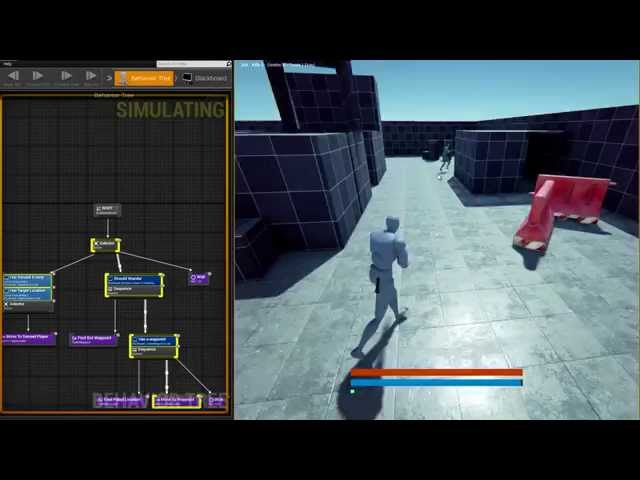
\includegraphics[width=\linewidth]{img/videogame_tree.jpg}
		\caption{Conception d'un jeu vidéo utilisant les BT}
		\label{fig:BT2}
	\end{figure}
	\\
	L'objectif de ce rapport est de faire une synthèse de l'utilisation émergente des BT en robotique, et ce dans de multiples domaines.
	\\
	Tout d'abord, nous allons définir ce qu'est un BT et quelles sont ses utilisations historiques. Ensuite, nous verrons qu'elles sont les nouvelles applications de cette technique dans les domaines variés de la robotique. Enfin, nous décrirons une implémentation simple d'un BT dans un projet de robotique théorique.
	
	\section{Qu'est-ce-qu'un behavior tree ?}
		\subsection{Définition}
		Un arbre de comportement est un modèle mathématique d'exécution de plans utilisé en informatique, en robotique, en systèmes de contrôle et dans les jeux vidéo. Ils décrivent les basculements entre un ensemble fini de tâches de manière modulaire. Leur force provient de leur capacité à créer des tâches très complexes composées de tâches simples, sans se soucier de la façon dont les tâches simples sont mises en œuvre. \cite{wikipedia_BT}
		\subsection{Fonctionnement}
		
		D'un point de vue conceptuel, un BT est basé sur deux objets clés : le nœud et l'arborescence.
		
		\begin{figure}[h!]
			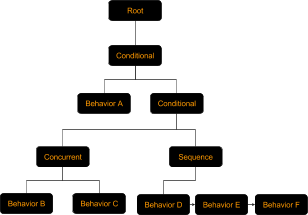
\includegraphics[width=\linewidth]{img/behavior_trees_example.png}
			\caption{exemple de BT \cite{rasmussen}}
			\label{fig:BT1}
		\end{figure}
		
		\paragraph{Nœud}
		Le nœud est le concept le plus fondamental ici. il s'agit d'un bloc de construction qui peut être associé à d'autres pour construire des comportements. Un nœud se compose d'un bloc de code qui représente une tâche simple. Tous les nœuds ont la même interface : lors de leur traitement, ils effectuent une tâche et peuvent réussir ou échouer.
		
		Les nœuds peuvent être autonomes ou avoir des nœuds enfants, lesquels sont traités dans le cadre du traitement du nœud parent. Lors du traitement, la réussite d'un nœud parent dépend souvent (mais pas toujours) de la réussite de chaque nœud enfant.
		
		Les nœuds suivent plusieurs modèles courants, tels que les nœuds d'action, composites et décorateurs. \cite{documentation_aws}
		
		\paragraph{Arborescence}
		Les comportements sont élaborés en construisant des arborescences de nœuds, collections de tâches individuelles qui, lorsqu'elles sont positionnées comme une racine avec des branches qui se terminent par des feuilles, définissent la façon dont un agent intelligent se comportera en réponse à une entrée. \cite{documentation_aws}	
		\subsection{Behavior Tree face à FSM et HFSM}
		Une machine à états finis (FSM) est un modèle mathématique de calcul. C'est une machine abstraite qui peut se trouver exactement dans un nombre fini d'états à un moment donné. Le FSM peut passer d'un état à un autre en réponse à certaines entrées externes; le passage d'un état à un autre s'appelle une transition. Un FSM est défini par une liste de ses états, son état initial et les conditions de chaque transition. \cite{wikipedia_FSM}
		\\
		D'après Colledanchise \cite{colledanchise_2017} d'un point de vue théorique, chaque exécution décrite par un BT peut être décrite par un FSM et inversement. Toutefois, en raison du nombre de transitions, l'utilisation d'un FSM en tant qu'architecture de contrôle n'est pas pratique pour certaines applications robotiques. De plus, un FSM suppose que les propositions qui déclenchent les transitions sortantes à partir du même état s’excluent mutuellement. Une fois mises en œuvre, les propositions sont vérifiées régulièrement en un temps discret. Il existe donc une probabilité que deux propositions ou plus se tiennent simultanément après un cycle. Pour résoudre ce problème, il faut redéfinir la signification de certaines transitions, afin de les rendre mutuellement exclusives. Un FSM de ce format est peu pratique à concevoir pour les humains et les ordinateurs. Ajouter et supprimer des comportements humains est sujet à des erreurs. Après avoir ajouté un nouvel état, chaque transition existante doit être réévaluée et les nouvelles transitions vers le nouvel état doivent également être évaluées. Un grand nombre de transitions rend tout processus automatisé d'analyse ou de synthèse coûteux en FSM.
		\\
		Les marchines à états finis hierarchique (HFSM) sont les autorités de certification les plus similaires aux BT en termes d'objectif et d'expressivité. Pour comparer les BT aux HFSM, veuillez vous référer aux schémas 3.8 et 3.9 de \cite{colledanchise_2017}. Une différence importante est que, dans les HFSM, chaque couche de la hiérarchie doit être ajoutée explicitement, alors que dans les BT, chaque sous-arbre peut être vu comme un module à part entière.
		\subsection{Historique}
			Les BT ont été développés dans l’industrie du jeu vidéo, en tant qu’outil pour accroître la modularité des structures de contrôle des PNJ. Dans cette industrie valant des milliards de dollars, la modularité est une propriété essentielle pour permettre la réutilisation du code, la conception incrémentielle des fonctionnalités et des tests efficaces. Les FSM deviennent de plus en plus difficiles à déboguer d'où l'apparition des BT. Damian Isla a expliqué cela en détail à propos de l’intelligence artificielle de Halo 2 lors de son exposé sur la GDC en 2005. \cite{gdc_2005}
			\\
			\begin{figure}[h!]
				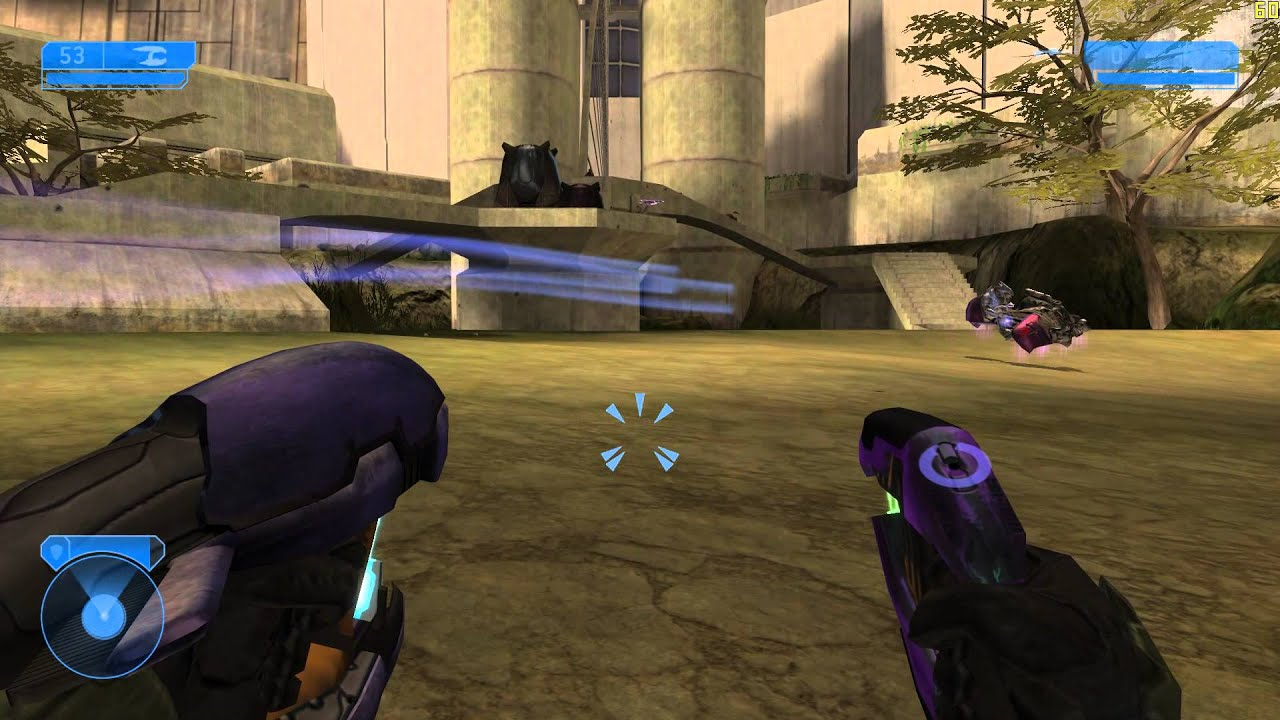
\includegraphics[width=\linewidth]{img/halo2.jpg}
				\caption{Le jeu vidéo Halo 2, un précurseur en matière d'intelligence artificielle dans le jeu vidéo grâce à son utilisation des BT \cite{wikipedia_halo}}
				\label{fig:BT1}
			\end{figure}
			\\
			Suite au développement de l'industrie du jeu vidéo, les BT ont également commencé à attirer l'attention du monde universitaire.
			\\
			À la Carnegie Mellon University, les BT ont été largement utilisés pour la manipulation robotique. La modularité est la principale raison de l'utilisation des BT. "L'avantage principal est que les comportements individuels peuvent facilement être réutilisés dans le contexte d'un autre comportement de niveau supérieur, sans qu'il soit nécessaire de spécifier leur relation avec les événements ultérieurs. comportements".\cite{Bagnell_2012_7606}
			\\
			D'après Colledanchise \cite{colledanchise_2017}, les BT ont également été utilisés pour permettre à des non-experts d’effectuer une programmation robotisée des opérations de sélection et d’emplacement, grâce à leur représentation modulaire et adaptable d’une tâche robotique. Ils ont également permis aux utilisateurs finaux de créer visuellement des programmes aussi complexes et puissant en tant que programmes écrits de manière traditionnelle. De plus, les BT ont été proposés comme composant clé de la robotique de chirurgie cérébrale en raison de "leur flexibilité, leur réutilisabilité et leur syntaxe simple".\cite{hu_gong_hannaford_seibel_2015}
	\clearpage
	\section{Les behavior tree en robotique}
		\subsection{Civil}
		\paragraph{Exemple}
		\begin{figure}[h!]
			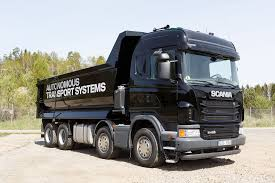
\includegraphics[width=\linewidth]{img/vehicul.jpg}
			\caption{Un poids lourd entièrement autonome iQmatic}
			\label{fig:civil}
		\end{figure}	
		iQmatic est un projet dirigé par Scania (constructeur de camions haut de gamme) qui vise à développer un véhicule (camion, autobus, etc.) pour le transport de marchandises, l’exploitation minière et d’autres applications industrielles. 
		\\
		Le logiciel du véhicule doit être réutilisable, maintenable et facile à développer. Pour ces raisons, les développeurs d’iQmatic ont choisi BT comme architecture de contrôle pour le projet.
		Les BT sont appréciés dans iQmatic pour leur lisibilité humaine, qui supportent la conception et le développement des premiers prototypes. La figure 4 montre un des camions utilisés dans le banc d’essai iQmatic
		\subsection{industrie}
		\paragraph{Exemple}
		\begin{figure}[h!]
			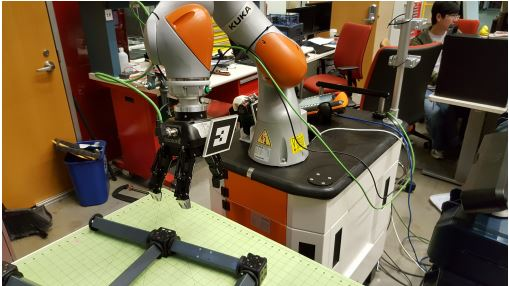
\includegraphics[width=\linewidth]{img/robotind.JPG}
			\caption{The CoSTAR project}
			\label{fig:civil}
		\end{figure}
		Costar est un projet qui vise à développer un logiciel qui contient des outils pour composer des plans de tâches et permettre aux robots de formation de répondre à des comportements complexes pour des applications industrielles impliquant la coopération humaine.
		Remplacer par LA PARTIE KTH
		
		\subsection{santé}
	prédire comportement
	
		\subsection{militaire}
	Robot Thales \cite{mer_et_marine_2018}.

	\section{Les outils implémentant les behavior trees}
		\subsection{outils utilisés}
			En examinant les logiciels disponibles pour la conception et l'exécution de FSM et de BT, nous constatons que les outils du côté FSM, tels que IBM Rhapsody 2 et Stateflow 3, sont beaucoup plus avancés. Néanmoins, de nombreuses plates-formes de développement de jeux informatiques, telles que Unity3d 4\cite{technologies} et Unreal Engine 5 \cite{unreal_engine}, disposent désormais d'outils permettant de travailler avec des BT. Pour ceux qui souhaitent mettre en œuvre leur propre cadre, nous notons que la mise en œuvre standard des FSM est assez simple, alors que les HFSM et les BT nécessitent davantage de considération. Cependant, les implémentations open source sont disponibles pour les deux.
			\\
			ROS est un de ces outils open source utilisé pour le développement de BT.
			La bibliothèque est accessible au public sur le site de ros \cite{ros.org} et le référentiel de développeur est disponible sur le github \cite{miccol_2018_dev}. Une version non ROS de la bibliothèque en C ++ est disponible sur le github \cite{miccol_2018}. La bibliothèque est actuellement l’implémentation de ROS BT la plus étoilée disponible dans GitHub.
			\\
			Le but de cette bibliothèque est d’offrir un paquetage ROS BT open source gratuit. L'utilisateur définit la structure arborescente et développe le code des leaf nodes pour leur exécution et leur préemption. Les leaf nodes peuvent être implémentés dans le même node ROS que l'arborescence principale ou en tant que node ROS externes. Les node ROS externes peuvent être implémentés à l'aide de C++ ou de Python.
			\\
			Cependant les outils de BT ne sont pas forcement complets car ils sont très récents sur cette technologie dans le domaine de la robotique. Ainsi les outils ne sont pas forcément assez mature sur ce sujet et peuvent comporter des bugs. De plus ils n'ont pas forcement une communauté très développé car les connaissances sont moindres comparé à la communauté bien établie des FSM, cela est bien sûr amené à changer dans le futur.
		\subsection{machine learning}
		Dans la définition originale de l’arbre de comportement, les sélecteurs choisiront l’un de leurs nœuds-enfants à valider. L’algorithme parcourant l'arbre de gauche à droite pour trouver le premier des noeuds pouvant être activé donne aux noeuds de gauche les poids les plus élevés. \cite{Fu2016/08}
		\\
		Cependant, une considération plus naturelle consiste à attacher le poids aux nœuds enfants. Les sélecteurs cochent leurs nœuds enfants conformément aux poids de haut en bas. Cependant, cela implique d'ajuster manuellement les valeurs de pondération pour le système. Ce qui implique beaucoup de main-d'œuvre et de ressources : c'est une tâche très compliquée et très lourde, pas vraiment immaginable sur un très gros projet. \cite{Fu2016/08}
		\\
	\begin{figure}[h!]
		\centering
		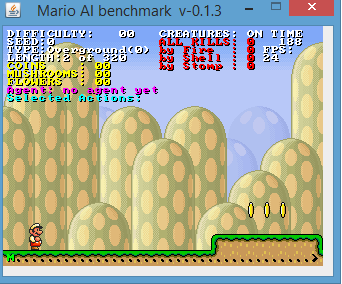
\includegraphics[width=200px]{img/mario-ai-benchmark.png}
		\caption{Mario AI Benchmark, un logiciel permettant de tester les solutions d'apprentissage machine}
		\label{fig:ai-benchmark}
	\end{figure}
		\\
		Une solution serait donc d'utiliser l'apprentissage machine (machine learning) afin de faire ajuster ces valeurs automatiquement. Cela à été testé avec Mario AI Benchmark par Colledanchise avec des résultats très encouragants et surtout supérieurs à ceux optenus avec un FSM plus classique (là encore entrainé avec du machine learning). \cite{colledanchise_2017}
	\section{Exemple}
	Pour notre exemple d'intégration, nous allons créer l'arbre comportemental d'un robot civil. Sa mission sera de remplacer les étudiants ayant du mal a se lever pour aller en cours. On ne s'intéressera pas à la conception (ni à la faisabilité) du dis robot, mais simplement à la modélisation de son comportement. 
	\\
	\begin{figure}[h!]
		\centering
		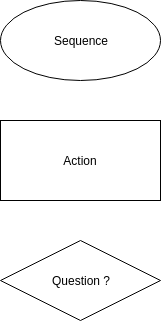
\includegraphics[width=50px]{img/BT_1.png}
		\caption{Nous utiliserons les symboles suivants pour modéliser notre BT}
		\label{fig:exemple_1}
	\end{figure}
	\\
	Tout d'abord, nous modélisons les blocs principaux du comportement, les trois phases de la mission du robot.
	\begin{enumerate}
		\item Phase de démarrage
		\item Journée de cours
		\item Arret
	\end{enumerate}
	En partant de ces 3 parties de la mission du robot, nous avons modélisé un arbre en utilisant une des propriétés les plus pratiques des arbres comportementaux : la modularité (la possibilité de modéliser les parties d'un arbre séparéments). \cite{iliffe_andrea_marlow_rachel_phillips_alexander_petter_2018}
	Nous avons donc décider de s'attribuer chacun une partie différente et de la développer séparément.
	\\
	\begin{figure}[h!]
		\centering
		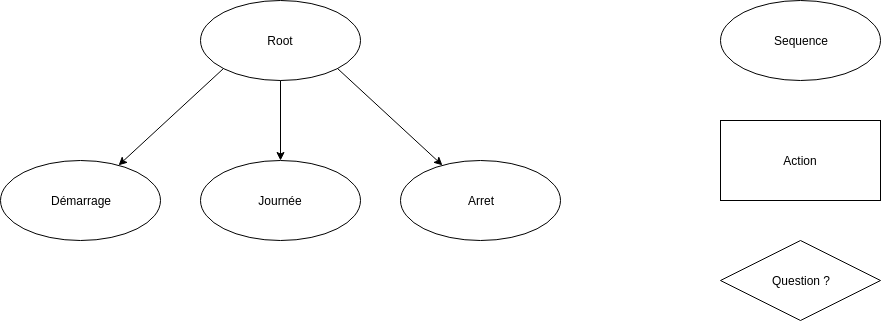
\includegraphics[width=\linewidth]{img/BT_2.png}
		\caption{Arbre après modélisation sommaire}
		\label{fig:exemple_2}
	\end{figure}
	\\
	\paragraph{Démarrage}
	C'est l'arbre de démarrage, qui est executé au départ du robot. Pour éviter que le robot parte en cours en même temps que l'élève, il a été décidé d'ajouter une validation manuelle. Pour aussi éviter que le robot ne parte avec un faible niveau de batterie, et se retrouve bloqué, on ajoute aussi une condition de démarrage.
	\paragraph{Journée}
	C'est l'arbre principal du robot. Il décrit le comportement pendant la journée. C'est son arbre de mission. Il comporte une référence à l'action "aller en cours", qui sera décrit plus tard.
	\paragraph{Arrêt}
	Cet arbre est très simple pour nous. Il ordonne au robot de retourner à sa base, son poste de stockage ou de rechargement.
	\\
	\begin{figure}[h!]
		\centering
		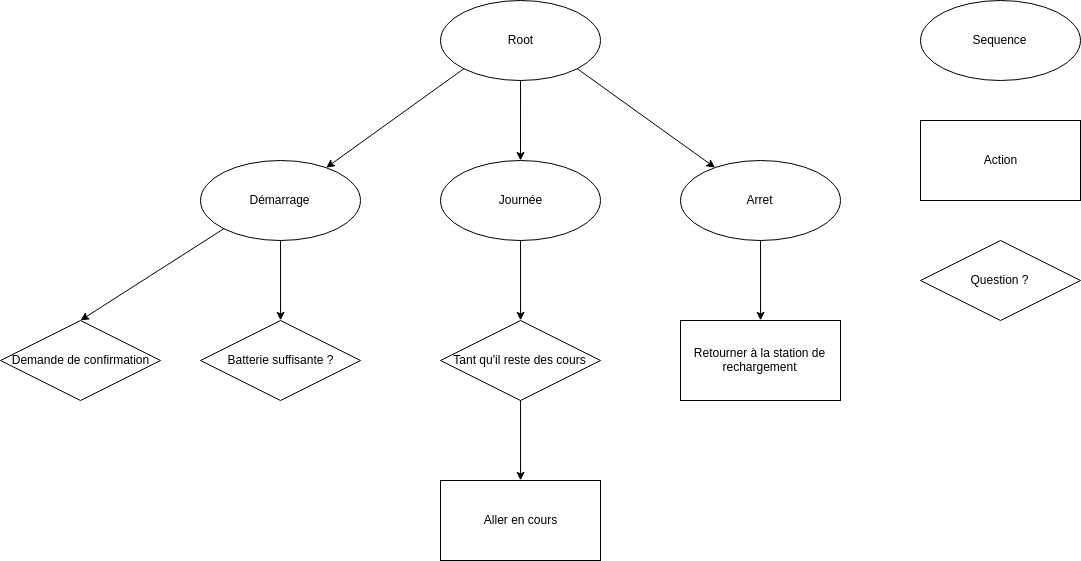
\includegraphics[width=\linewidth]{img/BT_4.png}
		\caption{Arbre après modélisation des arbres principaux}
		\label{fig:exemple_3}
	\end{figure}
	\paragraph{Aller en cours}
	Cet arbre est l'arbre le plus important du comportement, car il décrit la partie la plus sensible de la mission du robot.
	\begin{figure}[h!]
		\centering
		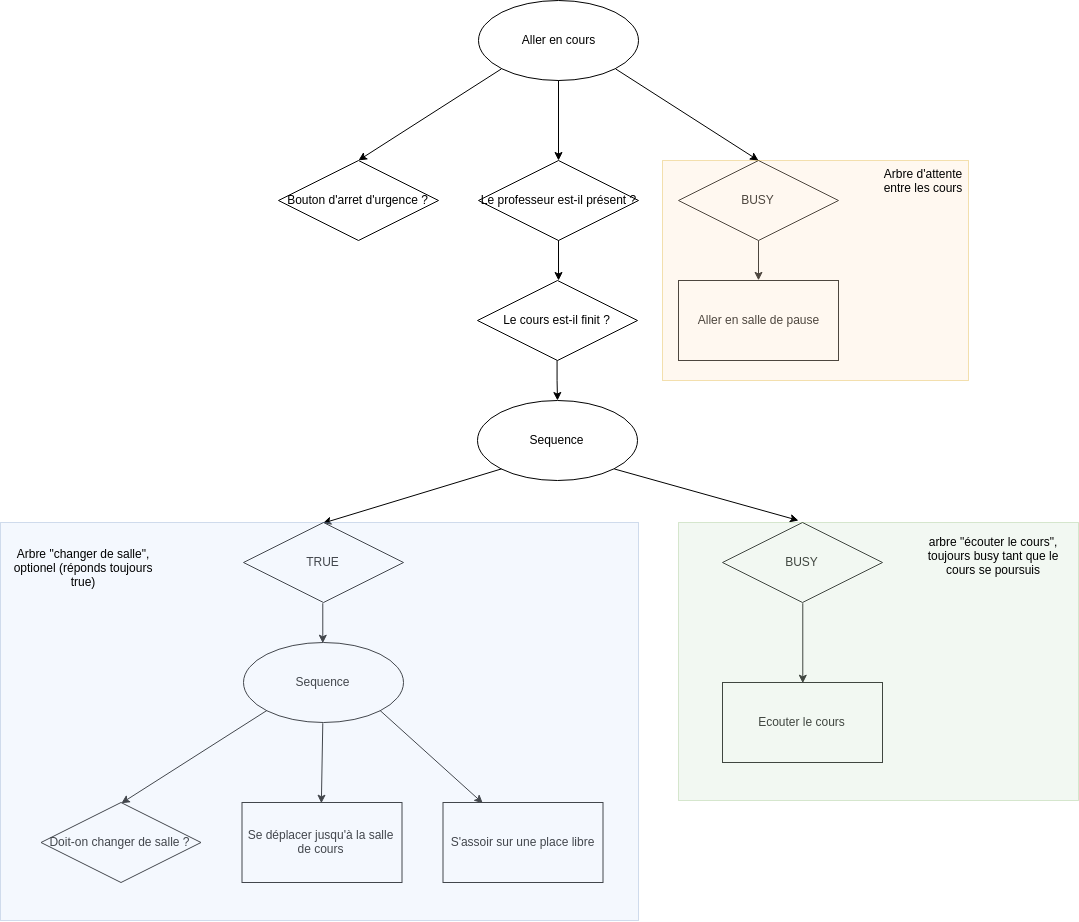
\includegraphics[width=\linewidth]{img/BT_5.png}
		\caption{Arbre "Aller en cours"}
		\label{fig:exemple_4}
	\end{figure}
	\\
	Pour modéliser le comportement, nous avons fait appel à des "décorateurs", des noeuds qui modifient simplement la réponses du reste de l'arbre mais éxécutent quand même leur propre arbre. 
	\\
	Par exemple, le décorateur "BUSY" force l'abre inférieur à toujours répondre BUSY, ce qui permet au robot de ne pas éxecuter le reste de l'arbre. Ce décorateur n'est pas réellement nécéssaire, mais permet d'augmenter la compatibilité de l'arbre avec d'autres actions qui répondrait parfois "TRUE" et executeraient une action indésirable. 
	\\
	Nous avons aussi ajouté un arbre "changer de salle", qui est totalement optionel. Il  évalue quand même son arbre mais finit toujours par répondre "TRUE" ou succès car son éxecution n'est pas requise systématiquement.
	\clearpage
	\section{Conclusion}
	Après avoir observé les outils et les implémentations existantes, nous pouvons tirer certaines conclusions sur l'utilisation des Behavior Tree en remplacement des FSM en robotique :
	\paragraph{Avantages} Les avantages des BT sont multiples: Tout d'abord, la modularité du système saute aux yeux. \cite{colledanchise_2017} Il est très facile de développer certaines branches séparément du reste de l'arbre comme nous l'avons montré dans notre exemple.
	Les BT sont aussi très adapté à l'utilisation du machine learning au sein même des arbres en modifiant les coefficients des actions. \cite{Fu2016/08}
	Aussi, compiler un BT permet de l'optimiser, évitant les problèmes de beaucoup d'autres CA (comme par exemple les FSM) qui sont très dépendants de leur design. \cite{colledanchise_2017}
	\paragraph{Inconvénients} Malgré tout, de nombreux problèmes subsistent : les BT sont loins d'une baguette magique. La technologie étant relativement récente, ni les développeurs ni les outils ne sont encore opérationnels à 100\%. Ces soucis peuvent rendre l'implémentation d'un BT couteuse par rapport à une FSM équivalente. \cite{colledanchise_2017} Cela est vrai en particulier pour les projets d'une taille relativement réduite. 
	De même, il convient de vérifier la pertinence d'une solution d'IA aussi avancé, dans certains environnement un système d'instructions simple est largement suffisant.
	\paragraph{Perspectives d'avenir} Le développement futur des BT est très lié à leur modularité. En effet, il est possible de développer de multiples actions et arbres de décisions séparément, en faisant appel aux experts des domaines concernés \cite{colledanchise_2017}. Il est aussi possible de tester chacunes des parties séparément (dans une simulation par exemple), permettant d'augmenter leur fiabilité. 
	\\
	Voyant toutes ces possibilitées, il n'est pas dur d'imaginer un futur fait d'arbres modulaires interchangeables permettant de piloter des robots eux aussi modulaires (ce qui est déjà le cas grâce à des logiciels comme ROS \cite{ros.org})
	\clearpage
	\section{Bibliographie}
	\bibliography{sources.bib}
	
\end{document}

